\documentclass[12pt,x11names,a4paper]{article}
\input{preamble}


\newgeometry{margin=2cm}

\pagestyle{fancy}
\fancyhf{}

\rhead{Nørre Gymnasium\\2.z
}
\cfoot{Side \thepage \hspace{1pt} af \pageref{LastPage}}

%Husk at rette modul og dato!
\lhead{Aflevering 3\\ Matematik B
}
\chead{8. november
}

\begin{document}

%\includepdf[pages=-]{Forsider/aarsprove_1v.pdf}
\savegeometry{art}

\begin{titlepage}
\newgeometry{margin=0pt}

\begin{minipage}{0.27\textwidth}

\begin{tikzpicture}[overlay]
\fill[top color = NorregGroen!40, bottom color = NorregGroen] (6,10) rectangle (-10,-30);
\end{tikzpicture}
\end{minipage}
\begin{minipage}{0.73\textwidth}
\begin{center}
\phantom{h} \vspace{1cm}\\
\hspace{4cm}
\includegraphics[scale = 1]{Billeder/Norreg.png} \\
\phantom{h} \vspace{5cm}\\
\rule{0.7\textwidth}{0.3mm}\\
\phantom{h}\\
{\fontsize{50}{60}\selectfont Aflevering 2}\\
\phantom{h}\\
\rule{0.7\textwidth}{0.3mm}\\
\Large 2024\\
\Large 2.z Ma

\end{center}
\end{minipage}
\end{titlepage}
\loadgeometry{art}

%Udfyld afsnit herunder og lav til egen Latex-fil

%Kopier følgende til overskrift:

%\begin{center}
%\Huge
%Aflevering 1
%\end{center}
%\section*{Opgave 1}
%\stepcounter{section}
\begin{center}
%Opgavesætter er delt i to dele:\\
%Delprøve 1 kun med den centralt udmeldte formelsamling.\\
%Delprøve 2 med alle hjælpemidler.
\end{center}

\section*{Krav til formidling af din besvarelse}

Ved bedømmelse af helhedsindtrykket af besvarelsen af de enkelte opgaver lægges særlig vægt på følgende fire punkter:
\begin{itemize}
\item[$\cdot$] \textbf{Redegørelse og dokumentation for metode} \\
Besvarelsen skal indeholde en redegørelse for den anvendte løsningsstragegi med dokumentation i form af et passende antal mellemregninger \textit{eller} matematiske forklaringer på metoden, når et matematisk værktøjsprogram anvendes.
\item[$\cdot$] \textbf{Figurer, grafer og andre illustrationer} \\
Besvarelsen skal indeholde hensigtsmæssig brug af figurer, grafer og andre illustrationer, og der skal være tydelige henvisninger til brug af disse i den forklarende tekst.
\item[$\cdot$] \textbf{Notation og layout}\\
Besvarelsen skal i overensstemmelse med god matematisk skik opstilles med hensigtsmæssig brug af symbolsprog, og med en redegørelse for den matematiske notation, der indføres og anvendes, og som ikke kan henføres stil standardviden.
\item[$\cdot$] \textbf{Formidling og forklaring}\\
Besvarelsen af rene matematikopgaver skal indeholde en angivelse af givne oplysninger og korte forklaringer knyttet til den anvendte løsningsstrategi beskrevet med brug af almindelig matematisk notation. 

Besvarelsen af opgaver, der omhandler matematiske modeller, skal indeholde en kort præsentation af modellens kontekst, herunder betydning af modellens parametre. De enkelte delspørgsmål skal afsluttes med en præcis konklusion præsenteret i et klart sprog i relation til konteksten.
\end{itemize}

\newpage

\begin{center}
\LARGE
Delprøve uden hjælpemidler 
\end{center}
\stepcounter{section}

%%%%%%%%%%%%%%%%%%%%%%%%%%
%
%
%
%
%%%%%%%%%%%%%%%%%%%%%%%%%%
\begin{opgavetekst}{Opgave 1}
	En funktion $f$ er givet ved
	\begin{align*}
		f(x) = 2x^3+4x^2-3x+6.
	\end{align*}
\end{opgavetekst}
\begin{delopgave}{}{1}
	Bestem $f(2)$.
\end{delopgave}
\begin{delopgave}{}{2}
	Bestem $f'(3)$.
\end{delopgave}
%%%%%%%%%%%%%%%%%%%%%%%%%%
%
%
%
%
%%%%%%%%%%%%%%%%%%%%%%%%%%
\begin{opgavetekst}{Opgave 2}
	En stykvist defineret funktion $g$ er givet ved
	\begin{align*}
		g(x) = \begin{cases}
			\log_5(x) \ &\textnormal{hvis }x \geq 0, \\
			x^2 \ &\textnormal{hvis }x < 0.		
		\end{cases}
	\end{align*}
\end{opgavetekst}
\begin{delopgave}{}{1}
	Bestem $g(125)$.
\end{delopgave}
%%%%%%%%%%%%%%%%%%%%%%%%%%
%
%
%
%
%%%%%%%%%%%%%%%%%%%%%%%%%%
\begin{opgavetekst}{Opgave 3}
	To vektorer $\vv{u}$ og $\vv{v}$ er givet ved
	\begin{align*}
		\vv{u} &= 
		\begin{pmatrix}
			3 \\ 4
		\end{pmatrix}, \\
		\vv{v} &= 
		\begin{pmatrix}
			7 \\ -2
		\end{pmatrix}
	\end{align*}
\end{opgavetekst}
\begin{delopgave}{}{1}
	Bestem arealet af det parallelogram, de to vektorer udspænder. 
\end{delopgave}
\begin{delopgave}{}{2}
	Bestem linjens ligning for linjen $l$, der går gennem punktet $(2,2)$ og som har $\vv{u}$ som 
	retningsvektor.
\end{delopgave}


\begin{opgavetekst}{Opgave 4}
	En funktion $h$ er givet ved
	\begin{align*}
		h(x) = \ln(x) + 3.
	\end{align*}
\end{opgavetekst}

\begin{delopgave}{}{1}
	Besten den afledede funktion for $h$. 
\end{delopgave}
\begin{delopgave}{}{2}
	Bestem ligningen for tangentlinjen, der går gennem punktet $(1,h(1))$.
\end{delopgave}

\begin{opgavetekst}{Opgave 5}
	Grafen for en eksponentialfunktion $f$ er givet ved Figur \ref{fig:eksp}.
	\begin{figure}[H]
		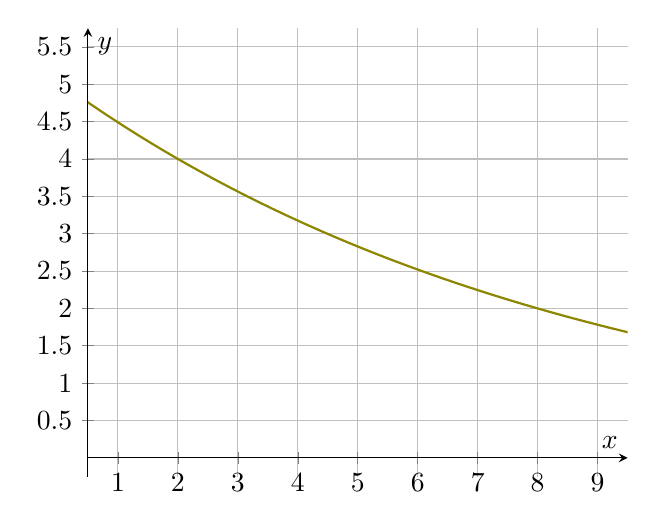
\begin{tikzpicture}
			\begin{axis}
			[axis lines = center, 
			xmin = 0.5, xmax = 9.5,
			ymin = -0.25, ymax = 5.75,
			grid = both, 
			xlabel = $x$,
			ylabel = $y$,
			xtick = {-1,0,...,9,10},
			ytick = {-1,-0.5,...,5,5.5},
			]
				\addplot[color = olive, thick, samples = 100, domain = -1:10] {5.0397*0.8909^x};
			\end{axis}
		\end{tikzpicture}
	\end{figure}
	\phantom{h}
\end{opgavetekst}
\end{document}




